% The figures in this section are rendered notebook outputs and should be
% regenerated from the parquet data before submission.

\section{Solar System Data Products}
\label{sec:ss-products}

\subsection{Overview}

The DP2 solar system data products concentrate on associations between Rubin
\texttt{DiaSource} observations and previously known objects.  These are
known-object products, not a blind moving-object search or an orbit catalog
derived from DP2 alone.  This release delivers observations whose positions
were associated with objects in the Minor Planet Center (MPC) orbit catalog,
as described in Section~\ref{sec:ss-association}, together with a
Rubin-derived catalog of object-level photometry, including per-band absolute
magnitudes, in the \texttt{SSObject} table.

Rubin also searched for and discovered new solar system objects in Prompt
Processing.  That discovery campaign preceded the official DP2 Data Release
processing so that newly reported objects entering the MPC catalog before the
cutoff could be treated as known objects during association.  Consequently,
objects first discovered by Rubin can occur in these products, but DP2 does
not deliver a standalone catalog of Rubin discoveries.  The Prompt Processing
discoveries will be described in a forthcoming series of papers, and future
Data Releases will deliver catalogs of Rubin discoveries.

DP2 provides five solar system tables (Table~\ref{tab:ss-tables}).  Two are
derived from the Rubin observations: \texttt{SSSource}\footnote{Rubin will
submit the astrometric measurements represented in \texttt{SSSource} to the
MPC in stages, allowing the association quality to be validated before each
submission and minimizing the risk of reporting misassociations.} contains
one row per associated detection and links measured \texttt{DiaSource}
photometry and astrometry to a predicted object, while \texttt{SSObject}
contains one row per object and summarizes its observations, per-band
photometric properties, and selected orbit-derived quantities.  The
Rubin-derived tables contain 8,149,633 \texttt{SSSource} rows for 299,819
distinct objects, with the same 299,819 objects represented in
\texttt{SSObject}.  Every \texttt{diaSourceId} occurs at most once.

% deluxetable's p{} column type is incompatible with array.sty >= v2.5
% combined with the lineno package (see AASJournals/AASTeX7#21); wrap
% long-text cells in a fixed-width \parbox instead of using a p{} column.
\newcommand{\wrapcell}[1]{\parbox[t]{0.55\textwidth}{#1}}
\begin{deluxetable*}{lrrl}
\tablecaption{Delivered DP2 Solar System Tables\label{tab:ss-tables}}
\tabletypesize{\footnotesize}
\tablewidth{0pt}
\tablehead{
\colhead{Table} & \colhead{Rows} & \colhead{Columns} &
\colhead{Intent and useful relations}}
\startdata
\texttt{SSSource} & 8,149,633 & 39 & \wrapcell{One row per associated
\texttt{DiaSource}, containing measured and predicted single-epoch
quantities.  Join by \texttt{diaSourceId} to the detection and by
\texttt{ssObjectId} or \texttt{designation} to object-level tables.} \\
\texttt{SSObject} & 299,819 & 80 & \wrapcell{One row per recovered known object,
including sampling summaries, phase-curve fits, and selected quantities
derived from the input orbit.} \\
\texttt{mpc\_orbits} & TBD\tablenotemark{a} & 53 & \wrapcell{MPC snapshot of
orbital elements, fit metadata, uncertainties, and MPC photometric
parameters.  The convenience \texttt{designation} column supports direct
joins to the Rubin-derived tables.} \\
\texttt{current\_identifications} & TBD\tablenotemark{a} & 11 & \wrapcell{MPC
mapping between primary and secondary provisional designations that refer to
the same physical object; useful for resolving aliases.} \\
\texttt{numbered\_identifications} & TBD\tablenotemark{a} & 11 & \wrapcell{MPC
mapping between permanent numbers and primary provisional designations, with
IAU designations, names, credits, and publication references where available.}
\\
\enddata
\tablenotetext{a}{Insert the row count from the final DP2 MPC snapshot.  The
source tables were not available to this drafting repository, and current
live-MPC counts would not describe the delivered snapshot.}
\end{deluxetable*}

The other three products are auxiliary snapshots of tables in the MPC
PostgreSQL database.  They provide reference catalogs for orbital information
and object cross-identification, retaining the upstream MPC semantics rather
than being recomputed from DP2 observations.  Their field definitions are
documented in the MPC schema for the PostgreSQL tables replicated through the
Small Bodies Node.\footnote{\url{https://docs.minorplanetcenter.net/mpc-ops-docs/data-and-services/replicated-tables-schema/}}
The \texttt{mpc\_orbits} table records the MPC orbit solution and associated
fit information for designated objects.  The
\texttt{current\_identifications} table identifies primary and secondary
provisional designations that refer to the same object, and
\texttt{numbered\_identifications} connects an object's permanent number to
its primary provisional designation.  The former includes both self-mappings
($A=A$) and links among aliases ($A=B$); the latter also carries IAU naming
information when available.  The \texttt{mpc\_orbits} table available at
ingestion did not contain comets.
Because the predictions used for association were generated from that
snapshot, no comets were available to be associated with DP2 detections and
none occur in the delivered \texttt{SSSource} or \texttt{SSObject} products.

In \texttt{SSSource}, \texttt{SSObject}, and \texttt{mpc\_orbits},
\texttt{designation} denotes the unpacked primary provisional designation of
the object.  This column was added to the delivered \texttt{mpc\_orbits} copy
as an end-user convenience; there it is identical, row by row, to
\texttt{unpacked\_primary\_provisional\_designation}.  It therefore provides
a readable and direct join key among \texttt{SSSource}, \texttt{SSObject},
and \texttt{mpc\_orbits}, without requiring users to unpack MPC designations.
For query performance, users should nevertheless prefer SQL joins on integer
identifiers such as \texttt{ssObjectId} wherever those identifiers are
available, and use \texttt{designation} for readability or when an
appropriate integer key is unavailable.

\subsection{Association and the \texttt{SSSource} Product}
\label{sec:ss-association}

The association input was a 2025 March 13 snapshot of the MPC orbit
database\footnote{Small bodies discovered after 2025 March 13---including those
found in Rubin data---are therefore absent from the \texttt{SSSource} table
delivered here.}, limited to objects whose observational arcs exceeded two
days.
Associations were made independently for each detector and visit using
positions predicted by Sorcha
\citep[][]{2025AJ....170..100M,2025AJ....170...97H} at the visit epoch from
this orbit catalog.
Predicted objects were first restricted to the detector footprint.  Measured
\texttt{DiaSource} coordinates were represented as unit vectors on the
celestial sphere and stored in a $k$-d tree.  For each predicted position, the
algorithm identified the nearest detection within $1\arcsec$.  Candidate
pairs were considered in increasing separation, accepting a pair only if
neither member had already been assigned.  Thus, this is a positional,
one-to-one match; it uses neither brightness, color, morphology, nor rate and
does not calculate a probabilistic association score.  The delivered
\texttt{diaDistanceRank} is set to one for every row and should not be used as
a measure of match ambiguity.  Chance associations remain possible because
the match does not use brightness or detection reliability, and are more
likely where the \texttt{DiaSource} density is high.  Users constructing a
high-purity sample should consider detection reliability, angular and
cross-track residuals, consistency with the predicted magnitude, and the
uncertainty of the input orbit.  Detection-level reliability information
requires the join to \texttt{DiaSource} described below.

Each accepted row carries the measured position and the Sorcha ephemeris
position, the measured PSF photometry and band, the predicted apparent
$V$-band magnitude, phase angle and solar elongation, heliocentric and
topocentric distances, sky-plane and radial rates, and Cartesian position and
velocity components.  R.A. and decl. are in degrees in the ICRS frame;
the observation epoch \texttt{DIA\_midpointMjdTai} is an MJD on the TAI time
scale.  Distances are reported in au, velocities in
$\mathrm{km\,s^{-1}}$, sky rates in $\mathrm{deg\,day^{-1}}$, and residuals
in arcseconds.  State vectors are equatorial and evaluated at the
light-emission (retarded) time.  External comparisons must convert DP2 TAI
epochs to the service's time scale; at a representative main-belt rate,
neglecting the 37~s TAI--UTC offset produces a $\sim0.23\arcsec$ shift.

\texttt{SSSource} is an association and ephemeris product rather than a copy
of the complete \texttt{DiaSource} record.  Although it contains selected
measured quantities, users requiring the full detection-level measurements
and quality information should join to \texttt{DiaSource} using
\texttt{diaSourceId}.  Each \texttt{diaSourceId} occurs at most once in
\texttt{SSSource}, while unassociated \texttt{DiaSource} detections have no
corresponding \texttt{SSSource} row.  The ephemeris coordinates and state
vectors in \texttt{SSSource} describe the predicted object at the observation
epoch and should not be interpreted as a Rubin-derived orbital solution.

The matched-position residuals are strongly concentrated inside the adopted
radius (Figure~\ref{fig:ss-astrometry}).  The median radial offset is
$0.071\arcsec$, while the median coordinate offsets are $-9.2$~mas in R.A.
and $-22.7$~mas in decl..  Only 30 of the 8.15 million associations have
offsets at or above $0.9999\arcsec$.  The along-track and cross-track
distributions are narrowly centered near zero, with medians of approximately
10 and 11~mas, respectively.  As an external check, one representative epoch
for each of 1000 well-determined, numbered asteroids was compared with JPL
Horizons.  Median separations were approximately 27~mas for the DP2 prediction
relative to JPL, 26~mas for Rubin relative to JPL, and 39~mas for Rubin
relative to the DP2 prediction.

A broader analysis of approximately 700,000 Rubin measurements of 65,000
known objects finds two regimes.  For long-observed objects discovered before
2000, the median measured-minus-predicted coordinate residuals are below
1~mas, with a scatter of approximately 13--14~mas, comparable to the
astrometric repeatability for bright stars.  Objects discovered during
2000--2020 show a different pattern: offsets relative to JPL Horizons are
spatially coherent across the DP2 footprint.  In $5\degr\times5\degr$ sky
cells, the median offset-vector length is approximately 19~mas, the 95th
percentile is approximately 30~mas, and the largest values approach 42~mas.
Our current hypothesis is that orbit catalogs can carry 20--40~mas systematic
errors in predicted positions, particularly in the southern hemisphere,
because many orbits were constrained primarily by northern, pre-Gaia
astrometry.  The effect appears to diminish for objects discovered in the
Gaia era.  This interpretation remains under investigation and will be
discussed in detail in a subsequent paper.

\begin{figure*}[t]
\centering
% Panels cropped from the six-panel rendered diagnostic in sssource_qc.ipynb.
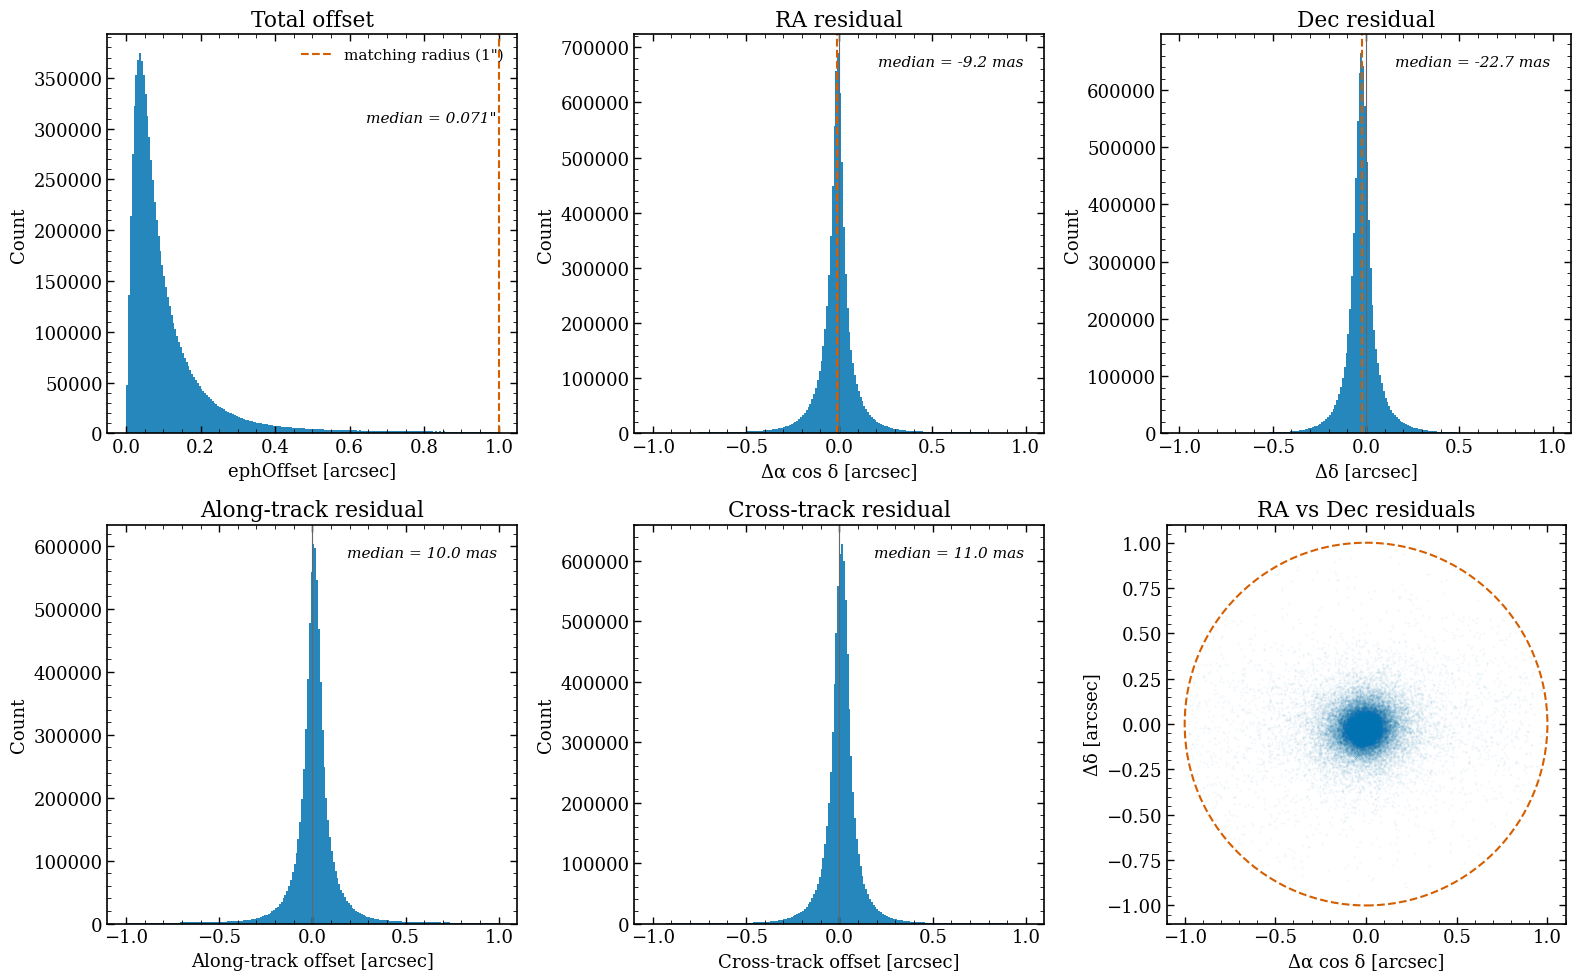
\includegraphics[width=0.40\textwidth,trim=0bp 350bp 740bp 0bp,clip]
    {figures/association_residuals.png}\hfill
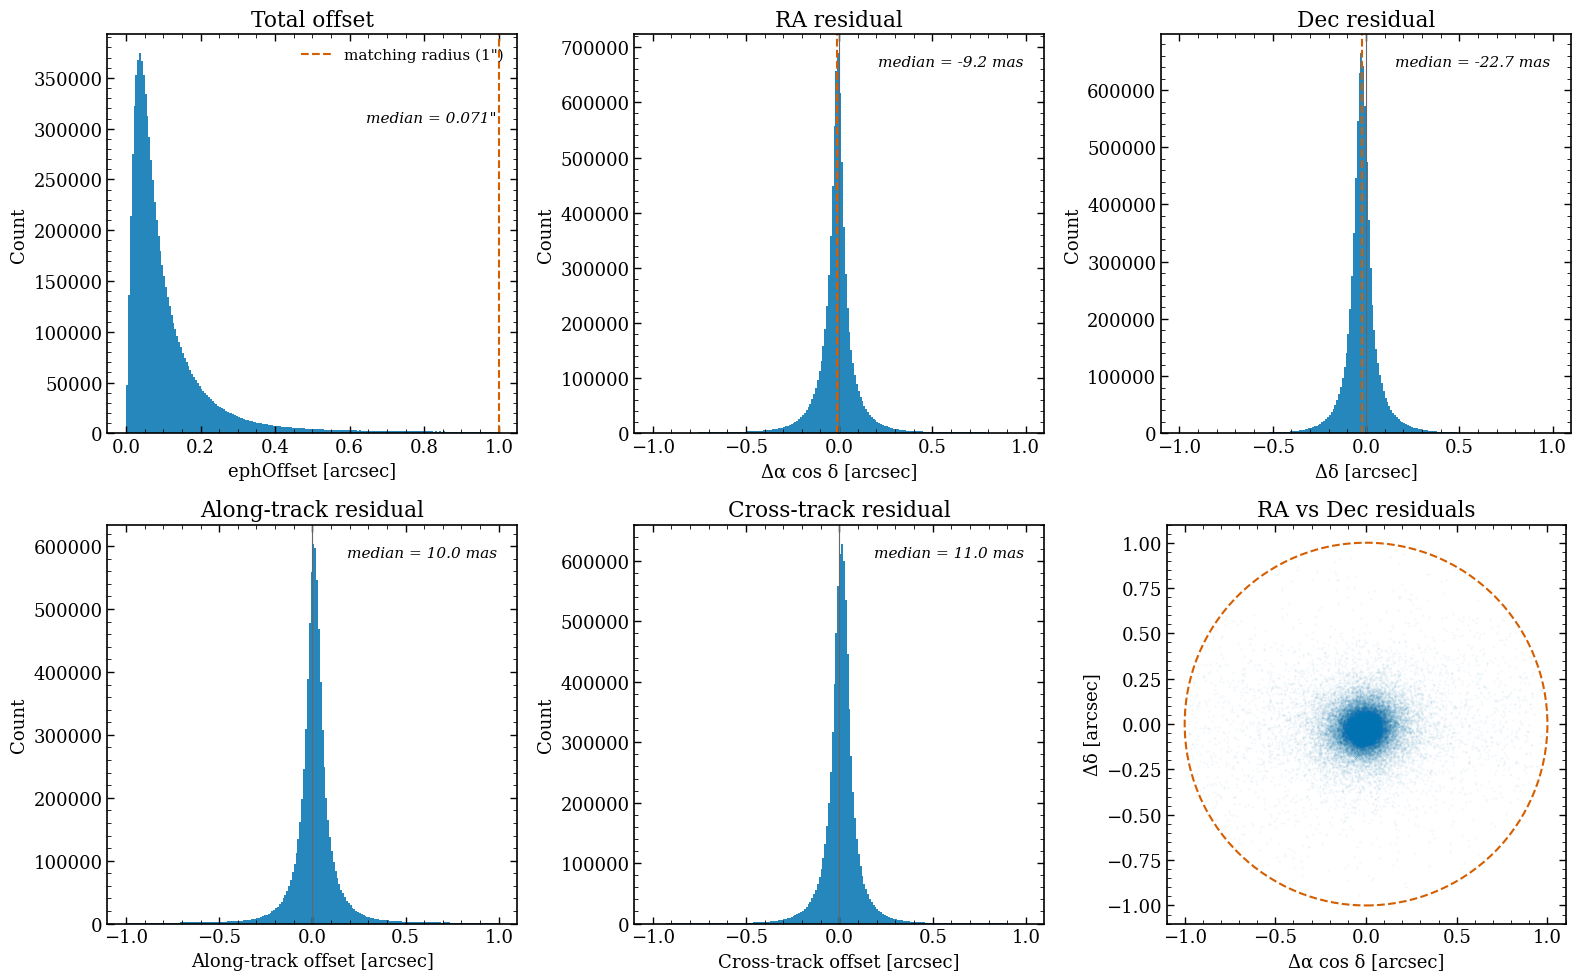
\includegraphics[width=0.40\textwidth,trim=800bp 0bp 0bp 360bp,clip]
    {figures/association_residuals.png}
\caption{Astrometric properties of the associations.  The distribution of
accepted angular separations (left) and measured-minus-predicted
R.A./decl. offsets for a reproducible random subset of 50,000
associations (right).  The dashed circle marks the $1\arcsec$ association
radius.  The raster panels are taken from the validation notebooks and will
be regenerated from the final parquet tables for publication.}
\label{fig:ss-astrometry}
\end{figure*}

The observations span a wide range of sampling and geometry.  There are
17,528 objects with a single associated detection, 31,873 with at most two,
212,181 with at least ten, and 7,293 with at least 100.  The main belt
dominates the distance and rate distributions, but the table includes 35
objects observed beyond 50~au, 765 source records at topocentric distances
below 0.1~au, and 2,105 records with predicted rates above
$1\mathrm{\,deg\,day^{-1}}$.  Its ecliptic-latitude range, $-69.4\degr$ to
$+13.3\degr$, primarily reflects the southern DP2 footprint rather than the
intrinsic solar system distribution.

The \texttt{ephVmag} field is an approximate predicted Johnson $V$ magnitude
derived from the input catalog photometric parameters.  It is not a prediction
in the Rubin band of the associated detection, so comparisons to the measured
$ugrizy$ photometry include both object color and phase-model differences
(Figure~\ref{fig:ss-photometry}).
One delivered record for 2015~GE86 has \texttt{ephVmag}$=104.6$ because the
input absolute magnitude was the MPC missing-value sentinel $H=99.99$; this
value should be treated as missing rather than physical.

\subsection{Object-level Photometry and Phase Curves}

The \texttt{SSObject} photometric fields were derived independently in each
of the $ugrizy$ bands from PSF fluxes in the associated detections.  For a
flux $f$ in nJy, the conversion used was
$m_{\rm AB}=31.4-2.5\log_{10}f$, with magnitude uncertainty
$1.085736\,\sigma_f/f$.  Non-positive fluxes therefore yield non-finite
magnitudes and were removed before fitting.  Apparent magnitudes were reduced
to unit heliocentric and topocentric distance using
$m(1,1,\alpha)=m-5\log_{10}(r\Delta)$, where $r$ and $\Delta$ are in au.

The reduced magnitudes were described with the $H,G_{12}$ phase function of
\citet[][]{2010Icar..209..542M}.  The DP2 processing fixed $G_{12}=0.5$ and fit only the
absolute magnitude $H$, since the short observing interval and limited
phase-angle coverage do not generally support a stable two-parameter fit.
Accordingly, valid per-band \texttt{G12} values are all 0.5, while
\texttt{G12Err} and the $H$--$G_{12}$ covariance are undefined.  A 0.05~mag
uncertainty floor was added in quadrature to the measurement uncertainties to
reduce sensitivity to unmodeled scatter, including rotational variability.
After removing non-finite magnitudes, an initial fit with a robust loss was
used to reject residuals beyond $10\sigma$, followed by a conventional
least-squares fit to the retained observations.  The per-band
\texttt{nObsUsed} field records the retained count and should be compared with
\texttt{nObs} when assessing clipping or invalid photometry.

Valid $H$ estimates were obtained for 35,268, 196,015, 224,888, 231,890,
203,341, and 90,789 objects in $ugrizy$, respectively.  Among objects with
sufficient observations for a fit, failures range from 53 in $y$ to 1,034 in
$g$, or less than approximately 0.5\% in every band.  Depending on band,
1--5\% of the eligible measurements were removed as invalid or clipped.
There are 25,706 objects with no fitted $H$ in any band; many are represented
by only one detection and hence have insufficient information for a fit.
The median fitted $H$ values are 18.7, 18.2, 17.5, 17.3, 17.2, and 16.6~mag
in $ugrizy$ (Figure~\ref{fig:ss-photometry}).  These distributions are
dominated by main-belt objects and are
also shaped by the DP2 footprint, cadence, phase-angle coverage, and
band-dependent detection selection; they should not be interpreted as
intrinsic population size distributions.

\begin{figure*}[t]
\centering
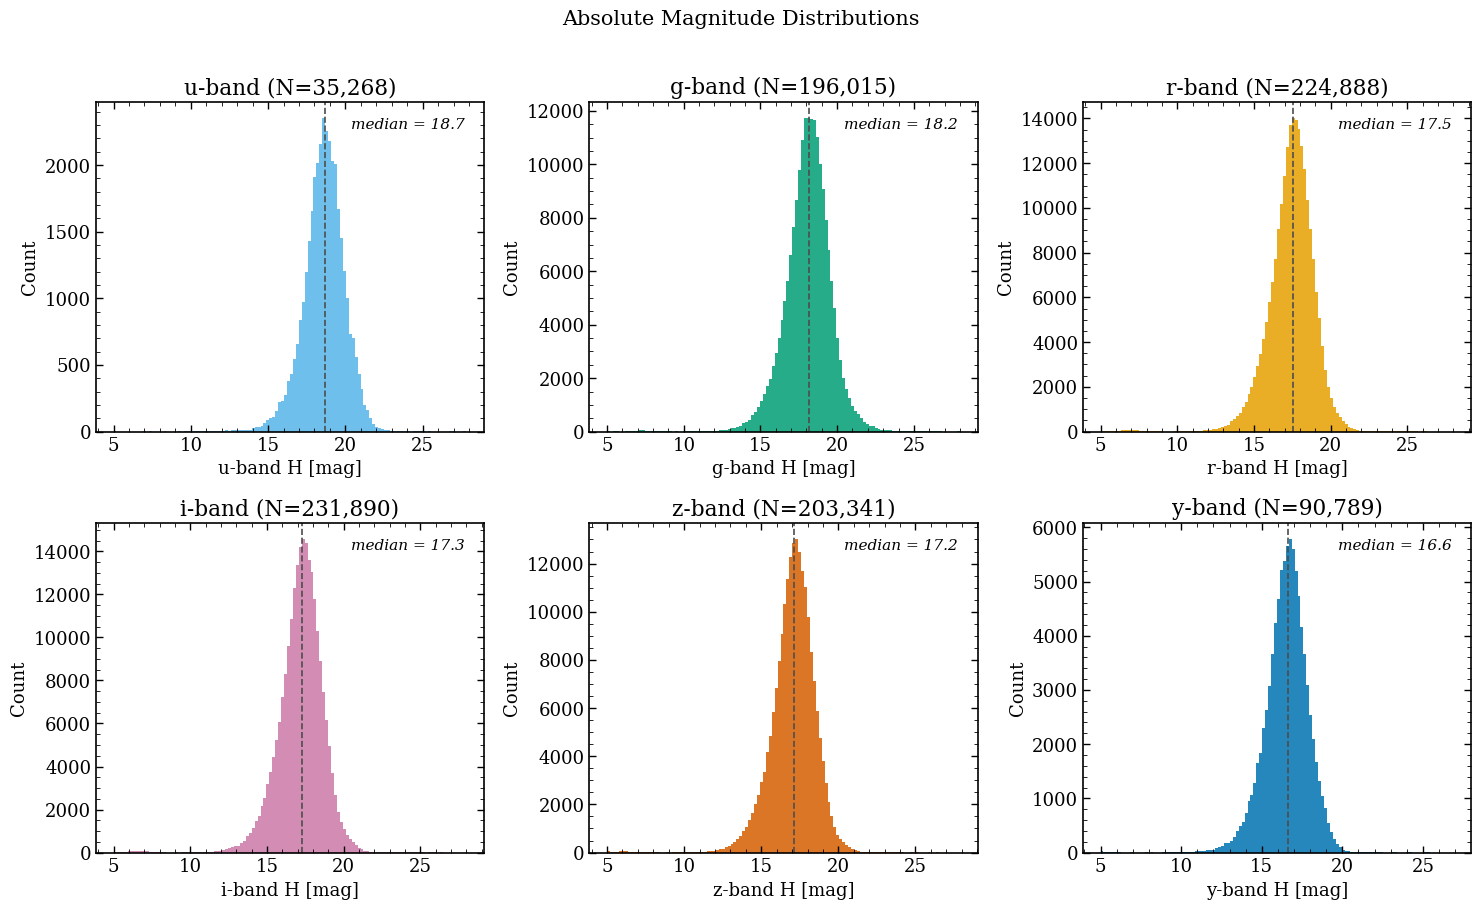
\includegraphics[width=0.68\textwidth]
    {figures/absolute_magnitude_distributions.png}

\vspace{3mm}
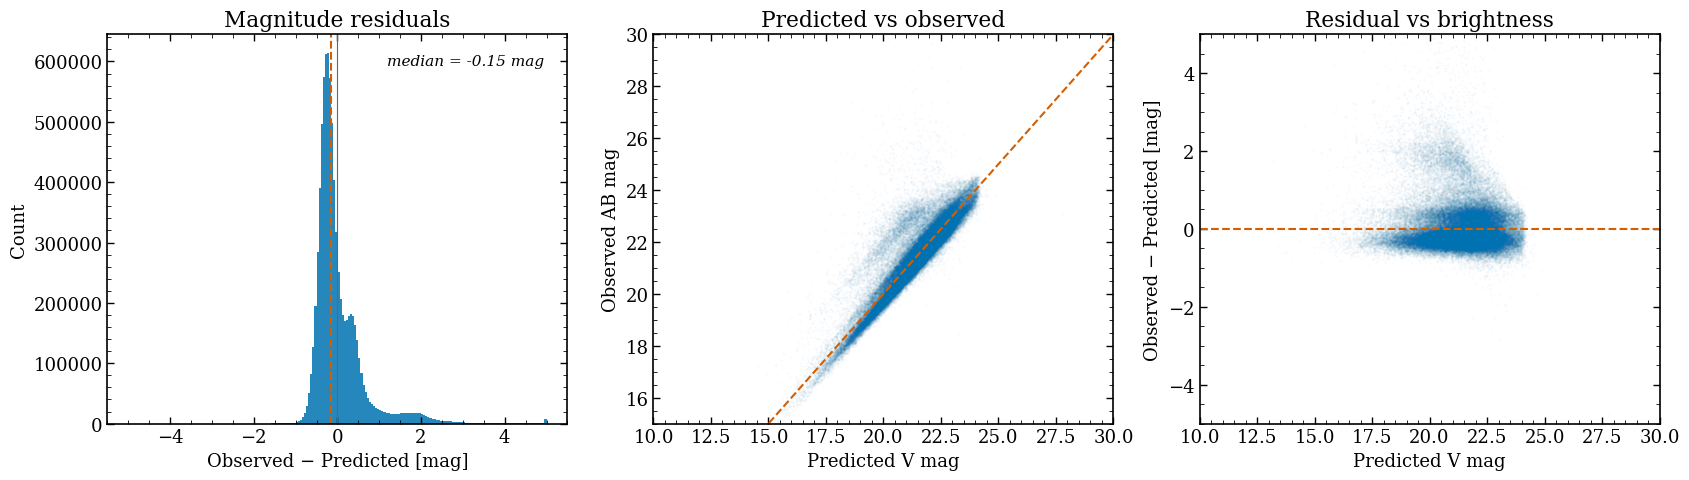
\includegraphics[width=0.98\textwidth]
    {figures/apparent_magnitude_diagnostics.png}
\caption{Photometric properties of the associations and fitted objects.
\emph{Top:} Per-band absolute-magnitude distributions; panel titles give the
number of valid fits and dashed lines mark the medians.  \emph{Bottom:}
Comparison of the measured apparent AB magnitude with the predicted Johnson
$V$ magnitude.  The left panel shows the observed-minus-predicted
distribution, the center panel the direct comparison, and the right panel the
residual as a function of predicted brightness.  The measured points combine
all six Rubin bands, so color terms, phase-model differences, and measurement
scatter all contribute; these panels are not a same-band photometric
calibration test.  The raster panels are taken from the validation notebooks
and will be regenerated from the final parquet tables for publication.}
\label{fig:ss-photometry}
\end{figure*}

The quoted \texttt{HErr} values are covariance-derived under the fixed
$G_{12}$ model and 0.05~mag error floor; they do not include uncertainty in
phase-function shape or a physical model of rotation.  Fits based on two or
three detections are more model-dependent than fits spanning many epochs and
a broad phase-angle range.  Users should therefore select on
\texttt{nObsUsed}, inspect \texttt{phaseAngleMin} and \texttt{phaseAngleMax},
and treat poor fits or discordant bands as possible signs of sparse sampling,
variability, blending, or misassociation.  A substantial high-value tail in
the per-band $\chi^2$ per degree of freedom likewise shows that the adopted
model and uncertainty floor do not capture all of the observed variability.
Moreover, observations in different bands were generally not simultaneous,
so colors formed from the fitted per-band $H$ values can include rotational
variability and should not be interpreted as instantaneous colors.

The resulting cross-band colors are broadly plausible for an asteroid sample:
the medians are approximately $g-r=0.58$, $r-i=0.18$, and $i-z=-0.01$~mag.
The tails are driven by sparse fits: of 721 objects with $|g-r|>3$~mag, 716
have only two to five $g$ observations and none has more than ten.  The phase
curves in Figure~\ref{fig:ss-phase-curves} show both mean phase dependence and
epoch-to-epoch scatter; fitted $H$ is not a rotationally resolved light curve.

\begin{figure*}[t]
\centering
% Retain the lower row of the rendered six-object phase-curve diagnostic.
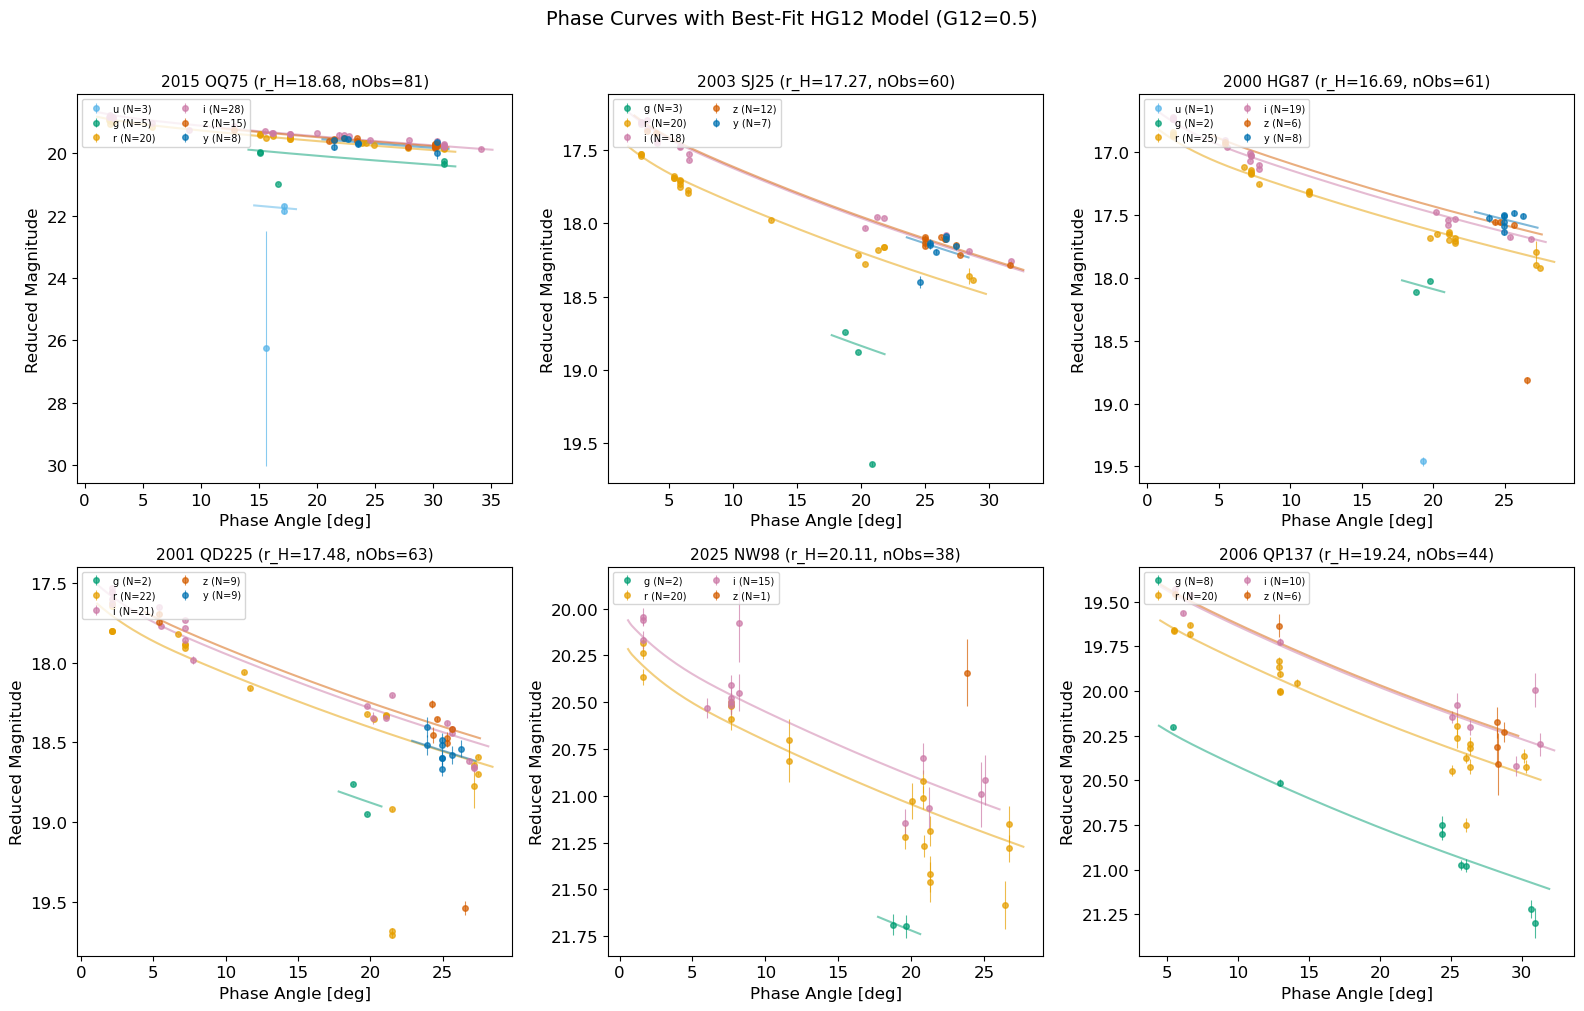
\includegraphics[width=0.92\textwidth,trim=35bp 5bp 8bp 415bp,clip]
    {figures/phase_curves.png}
\caption{Example distance-reduced phase curves for 2001~QD225,
2025~NW98, and 2006~QP137 (left to right), with observations colored by band
and the corresponding fixed-$G_{12}=0.5$ models shown as solid lines.  These
raster panels are taken from the validation notebooks and will be regenerated
from the final parquet tables for publication.}
\label{fig:ss-phase-curves}
\end{figure*}

\subsection{Other \texttt{SSObject} Fields and Usage Considerations}

In addition to the photometric fit outputs, \texttt{SSObject} records the
total and per-band observation counts, first observation epoch, observing
arc, per-band phase-angle limits, and extendedness summaries.  Although most
objects are point-like, 14,663 (4.9\%) have median extendedness of at least
0.5.  Its weak correlation with predicted rate means that a high value need
not imply trailing; blending and low-signal-to-noise classification can also
contribute.

The table also includes the Tisserand parameter with respect to Jupiter and
Earth minimum orbit intersection distance (MOID) quantities computed from the
input MPC orbital elements.  DP2 does not refit object orbits from the Rubin
observations.  The MOID calculation uses Earth elements evaluated at each
object's osculating epoch.  For 67,246 objects with a comparison value in the
MPC catalog, the median DP2-minus-MPC difference is approximately 0.1~mau and
65.4\% agree within 0.001~au.  Discrepancies can reach about 0.003~au among
objects with very small MOID, however, and the supplied values should not be
used by themselves for hazard classification or close-approach prediction.

For most analyses, \texttt{SSObject} is the starting point for cuts on count,
arc, phase coverage, and fit quality; join by \texttt{ssObjectId} for
epoch-level \texttt{SSSource} quantities.  Residual studies must account for
the hard $1\arcsec$ truncation, and population studies for the input catalog,
footprint, cadence, and difference-image detection.  These are product
selection effects, not properties of the underlying population.
